\documentclass{article}
\usepackage{fullpage, url,graphics, graphicx}
\usepackage{longtable}

\begin{document}
\title{Final Project: The Politics of Routing - Investigating the Link Between
Interdomain Connectivity and Internet Freedom}
\author{Hyungjoon Koo, Fahimeh Mirhaj and Rachee Singh}
\maketitle

\section*{Part 1: Data collection and analysis}

\bigskip

\noindent 
We have used the registered country code according to ISO3166-1. Currently $249$
country codes are officially available. The CAIDA data contains $51,501$ AS
numbers (ASN) all over the world. ~\ref{caida}
\bigskip

\noindent 
In order to map each ASN to the country, we leverage the registration
information provided by \texttt{cymru.com}. Out of all ASN, $50,818$ ASes can be
identified and $683$ ASes remained unidentified due to either missing or
inaccurate information. For example, the country code EU belongs to Europe, but
not a single country. Likewise, the code ZZ means the reserved ASN although the
ASN was shown in CAIDA. However, in this project, those connections have been
ignored which ended up with accounting for only $0.01\%$.
\bigskip

\noindent 
Along with ASN links from CAIDA, we combined the hidden edges using seperate
traceroute data, discovered by Rachee, with the existing links. As CAIDA data itself is
incomplete because it might not see the local edges, the combination of two data
set helps to get close to complete AS graphs. The number of connections among
ASes in CAIDA is $199,539$ as of Aug. 2015, and the number from traceroute data 
is $15,954$, thus we eventually gained $50,818$ nodes (ASes) and $215,493$ edges 
(links) in total for the entire graph. In the graph, blue nodes represents 
domestic ASes and red ones depicts international ASes.

\begin{figure}[h]

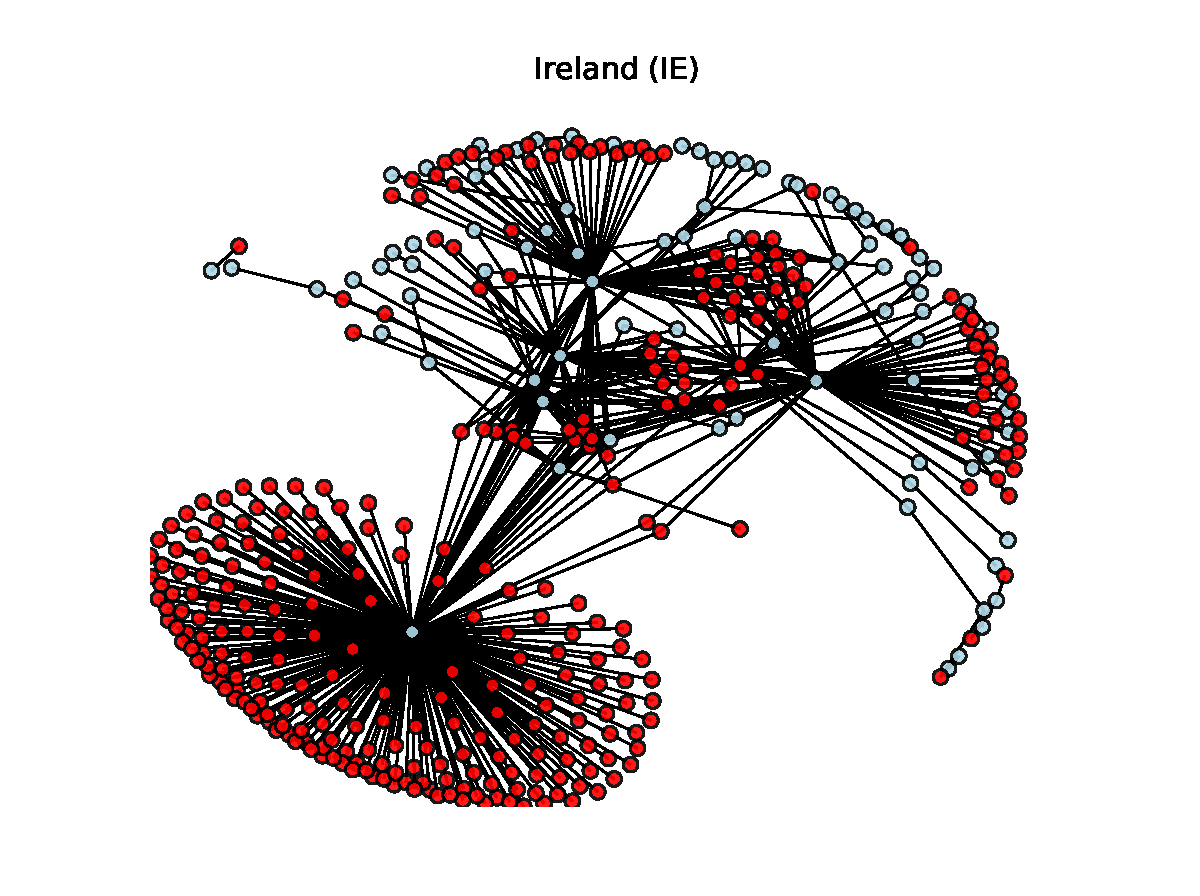
\includegraphics[width=0.8\linewidth]{IE.pdf}
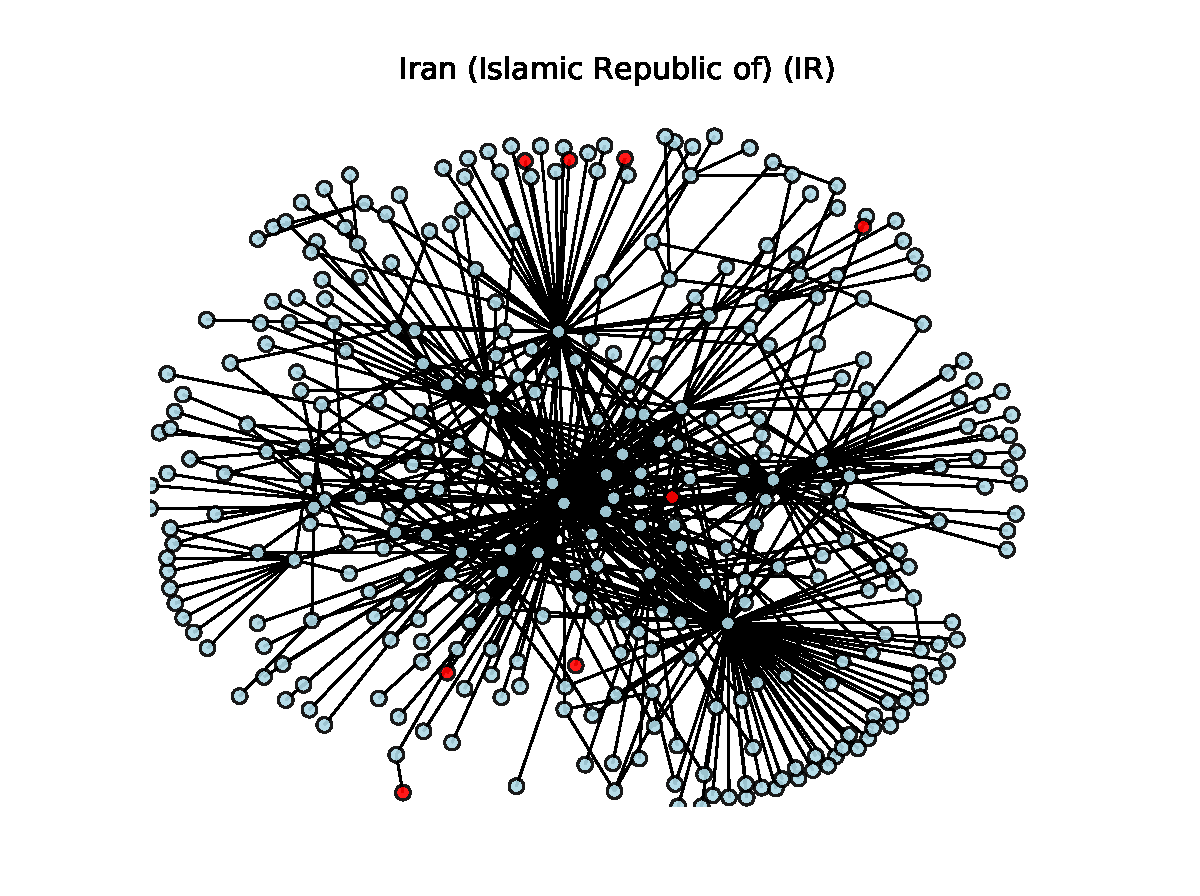
\includegraphics[width=0.8\linewidth]{IR.pdf}
\caption{The topology of Internet connectivity in Iran shows that only a few 
domestic ASes are connected to foreign ASes. This allows the country to control
the incoming and outgoing traffic flow easily. In contrast, the connectivity in Ireland
looks different, it is not known to have censorship operation. Ireland has many ASes
that connect to foreign countries (red circles).}
\label{fig:topo_iran}
\end{figure}

\section*{Part 2: Sub-graphs of the topology per each country}

\bigskip

\noindent 
The $231$ countries turn out to possess at least one or more ASes. First, we
produce the sub-graphs of the Internet topology for each country.
(http://dandylife.net/test/topologies) The graph illustrates what the topology
of $192$ countries looks like at a glance. Again, due to the incompleteness of
data set some edges are clearly missing, or some countries have no outgoing
connection. Figure~\ref{fig:topo_iran} illustrates the example of the topology 
for Iran that is known to censor Internet traffic. 


\section*{Part 3: Exploring the metrics}

\bigskip

\begin{table}[ht]
\centering
\caption{Correlationship Coefficient between each metric and public indexes}
\label{tab:corrcoeff}
\begin{tabular}{|l|l|l|l|}
\hline
\textbf{Explored Metrics}                              & \textbf{FHI} & \textbf{DI} & \textbf{RWBI} \\ \hline
Number of nodes                                        & 0.148157     & 0.153996    & 0.072192      \\ \hline
Number of edges                                        & 0.137037     & 0.142764    & 0.06467       \\ \hline
Number of foreign ASes *                                & 0.319965     & 0.320038    & 0.237468      \\ \hline
Number of domestic ASes connected to foreign ASes *      & 0.280964     & 0.296195    & 0.193413      \\ \hline
Average clustering coefficient                         & 0.155442     & 0.22917     & -0.0155       \\ \hline
Average degree connectivity                            & 0.208344     & 0.290089    & 0.11854       \\ \hline
Average neighbor degree                                & 0.24887      & 0.335812    & 0.13519       \\ \hline
Average node connectivity                              & 0.13002      & 0.172013    & -0.0176       \\ \hline
Surveillance index                                     & 0.085757     & 0.062251    & 0.112105      \\ \hline
Average shortest path length *                          & 0.384775     & 0.45908     & 0.255431      \\ \hline
Center                                                 & -0.12796     & -0.19907    & -0.00313      \\ \hline
Diameter *                                              & 0.419671     & 0.479558    & 0.284273      \\ \hline
Eccentricity                                           & 0.400835     & 0.461213    & 0.271562      \\ \hline
Periphery                                              & -0.07819     & -0.04564    & -0.04058      \\ \hline
Radius *                                               & 0.31978      & 0.365964    & 0.227006      \\ \hline
Density *                                               & -0.32574     & -0.42206    & -0.16544      \\ \hline
Components                                             & 0.426518     & 0.450295    & 0.350895      \\ \hline
Average Degree *                                        & 0.303342     & 0.377229    & 0.161176      \\ \hline
Average Path Length *                                   & 0.378565     & 0.45397     & 0.237122      \\ \hline
Modularity *                                            & 0.305919     & 0.419153    & 0.217303      \\ \hline
Community Number *                                      & 0.416936     & 0.492711    & 0.285289      \\ \hline
Total  Triangles                                       & 0.060901     & 0.106298    & 0.031786      \\ \hline
\end{tabular}
\end{table}

\noindent 
The goal of this project is to see how interdomain connectivity relates to
Internet freedom or economic/political characteristics of the countries based on
their interdomain connectivity. Therefore it is essential to choose appropriate
metrics and check how well they could explain the relationship bewteen AS
connectivity and Internet freedom. We have taken advantage of three official
indexes to measure economic/political characteristics: Freedom House Index (FHI),
Democracy Index (DI), and Reporters Without Borders Index (RWBI). However, not
all countries are available to get the indexes. We could obtain 192, 167, and
178 indexes (FHI in 2012, DI in 2014, and RWBI in 2015 in order) for different
country set respectively. The intersection of three indexes filters the final
131 countries to evaluate the metrics.

\bigskip

\noindent 
Each index represents different scale and meaning, thus we normalized and
tweaked it for consistency. For example, the lower index of both FHI and RWBI,
the better, which means the country with the low index has more freedom and less
censored country. Meanwhile, the higher DI represents the more developed country
in terms of democracy. Therefore, we normalized them from 0 to 1 that always
indicates 0 is the worst and 1 is the opposite. After adjusting the indexes, the
correlationship coefficients among them are 0.916, 0.797, and 0.877
respectively. (FH and DI, DI and RWBI, and FH and RWBI) This means these indexes
can be good indicator candidates to achieve the objective of this project.
Figure~\ref{fig:index_cdf} shows two cumulative distribution function (CDF) graphs. 
The first one is the distribution of ASes (nodes) and their links (edges), and the number
of ASes that have connection to foreign countries. The other one shows the distribution
of three publicly available indexes to explain the degree of freedom and democracy.

\bigskip

\noindent
Table~\ref{tab:data} is the part of the indexes and the number of ASes for a 
country.  After getting the sub-graphs of each country, in Table~\ref{tab:corrcoeff},
we have explored 22 different metrics with the help of both \texttt{networkX} and 
\texttt{gephi} libraries.

\begin{figure}[h]
\centering 
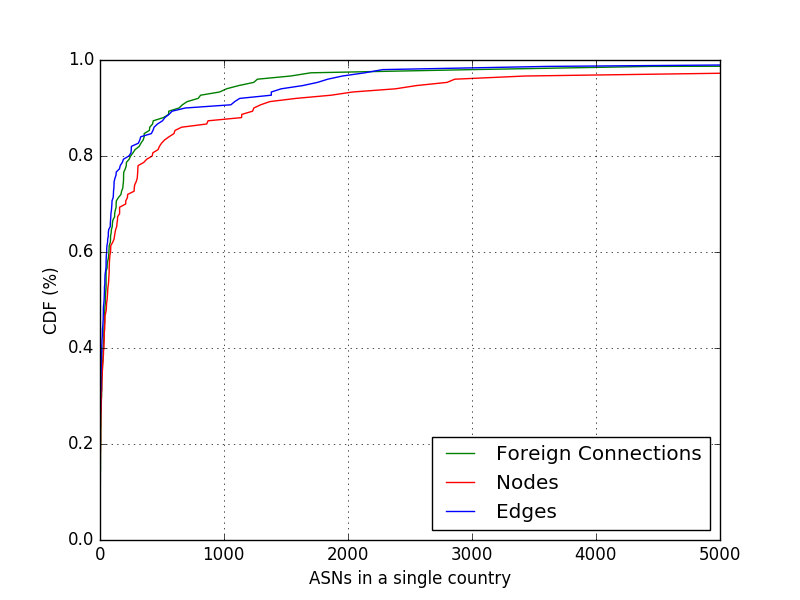
\includegraphics[width=0.8\columnwidth]{node_edge_foreign.png}
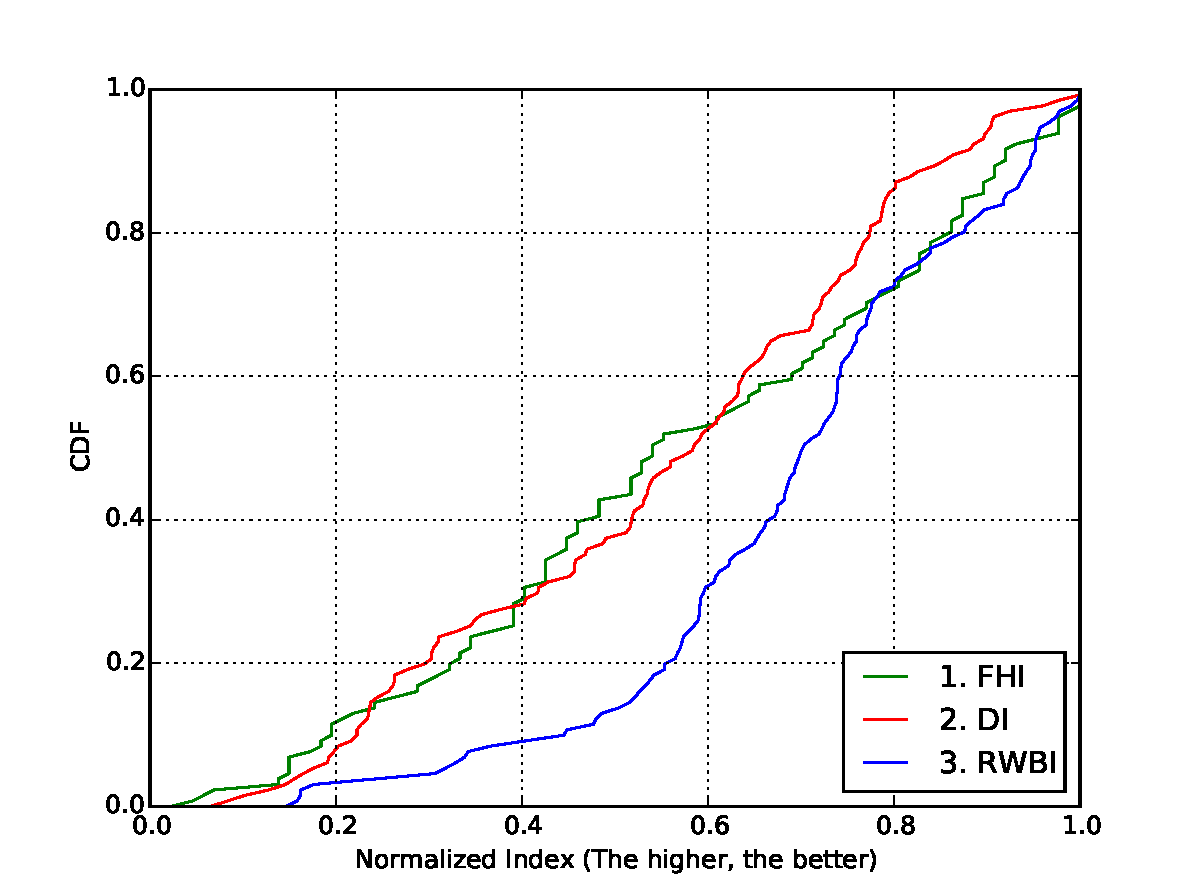
\includegraphics[width=0.8\columnwidth]{index_cdf.pdf}
\caption{The CDF of the Indexes - FHI, DI and RWBI}
\label{fig:index_cdf}
\end{figure}

\bigskip

\noindent
Note that correlationship coefficient is the coefficient that measures
statistical relationships quantitatively, such as correlation and dependence,
between two or more random variables or observed data values. It ranges from
$-1$ to $1$ that indicates two variables have either positive or negative
relationship. Once getting all values of the metrics for all countries, we
compute the correlationship coefficient between individual metric and the index.
Here we only care the case that the absolute value of the coefficient is larger than
$0.25$.

\bigskip

\noindent
We selected 10 metrics as the features for clustering. In Figure~\ref{fig:im_scatter},
the upper half consists of three rows and ten columns. Each scattering plot implies the 
positive or negative relationship between the metric and the index. Similarly, the lower 
half shows the CDF of each scattering that represents the relationship according to
the correlationship coefficients we discovered. Figure~\ref{fig:clustering} is the final
outcome of clustering with setting up 4 clusters as a parameter. We have evaluated
8 different clustering algorithm and each has different result. This is very expecting 
consequence because different clustering algorithms have their own strengths and
weaknesses. It is worth noting the there are several algorithms that automatically decide
the number of possible clusters. Different colors represent different clusters,
and each dot means a single country. If the algorithm needs the parameter, we separately
marked it on the bottom of each clustering. 
In particular, K-means algorithm found the centroid of each cluster that has been marked
as large circle in the figure.

\bigskip

\noindent
We have not combined all features together when performing clustering, because we were
not able to discover the feature that strongly supports the relationship between ASN and 
the freedom of Internet or the degree of democracy for a country. It is still an open problem,
but this project sheds light on the possibility of the relationship.

\begin{figure}[h]
\centering 
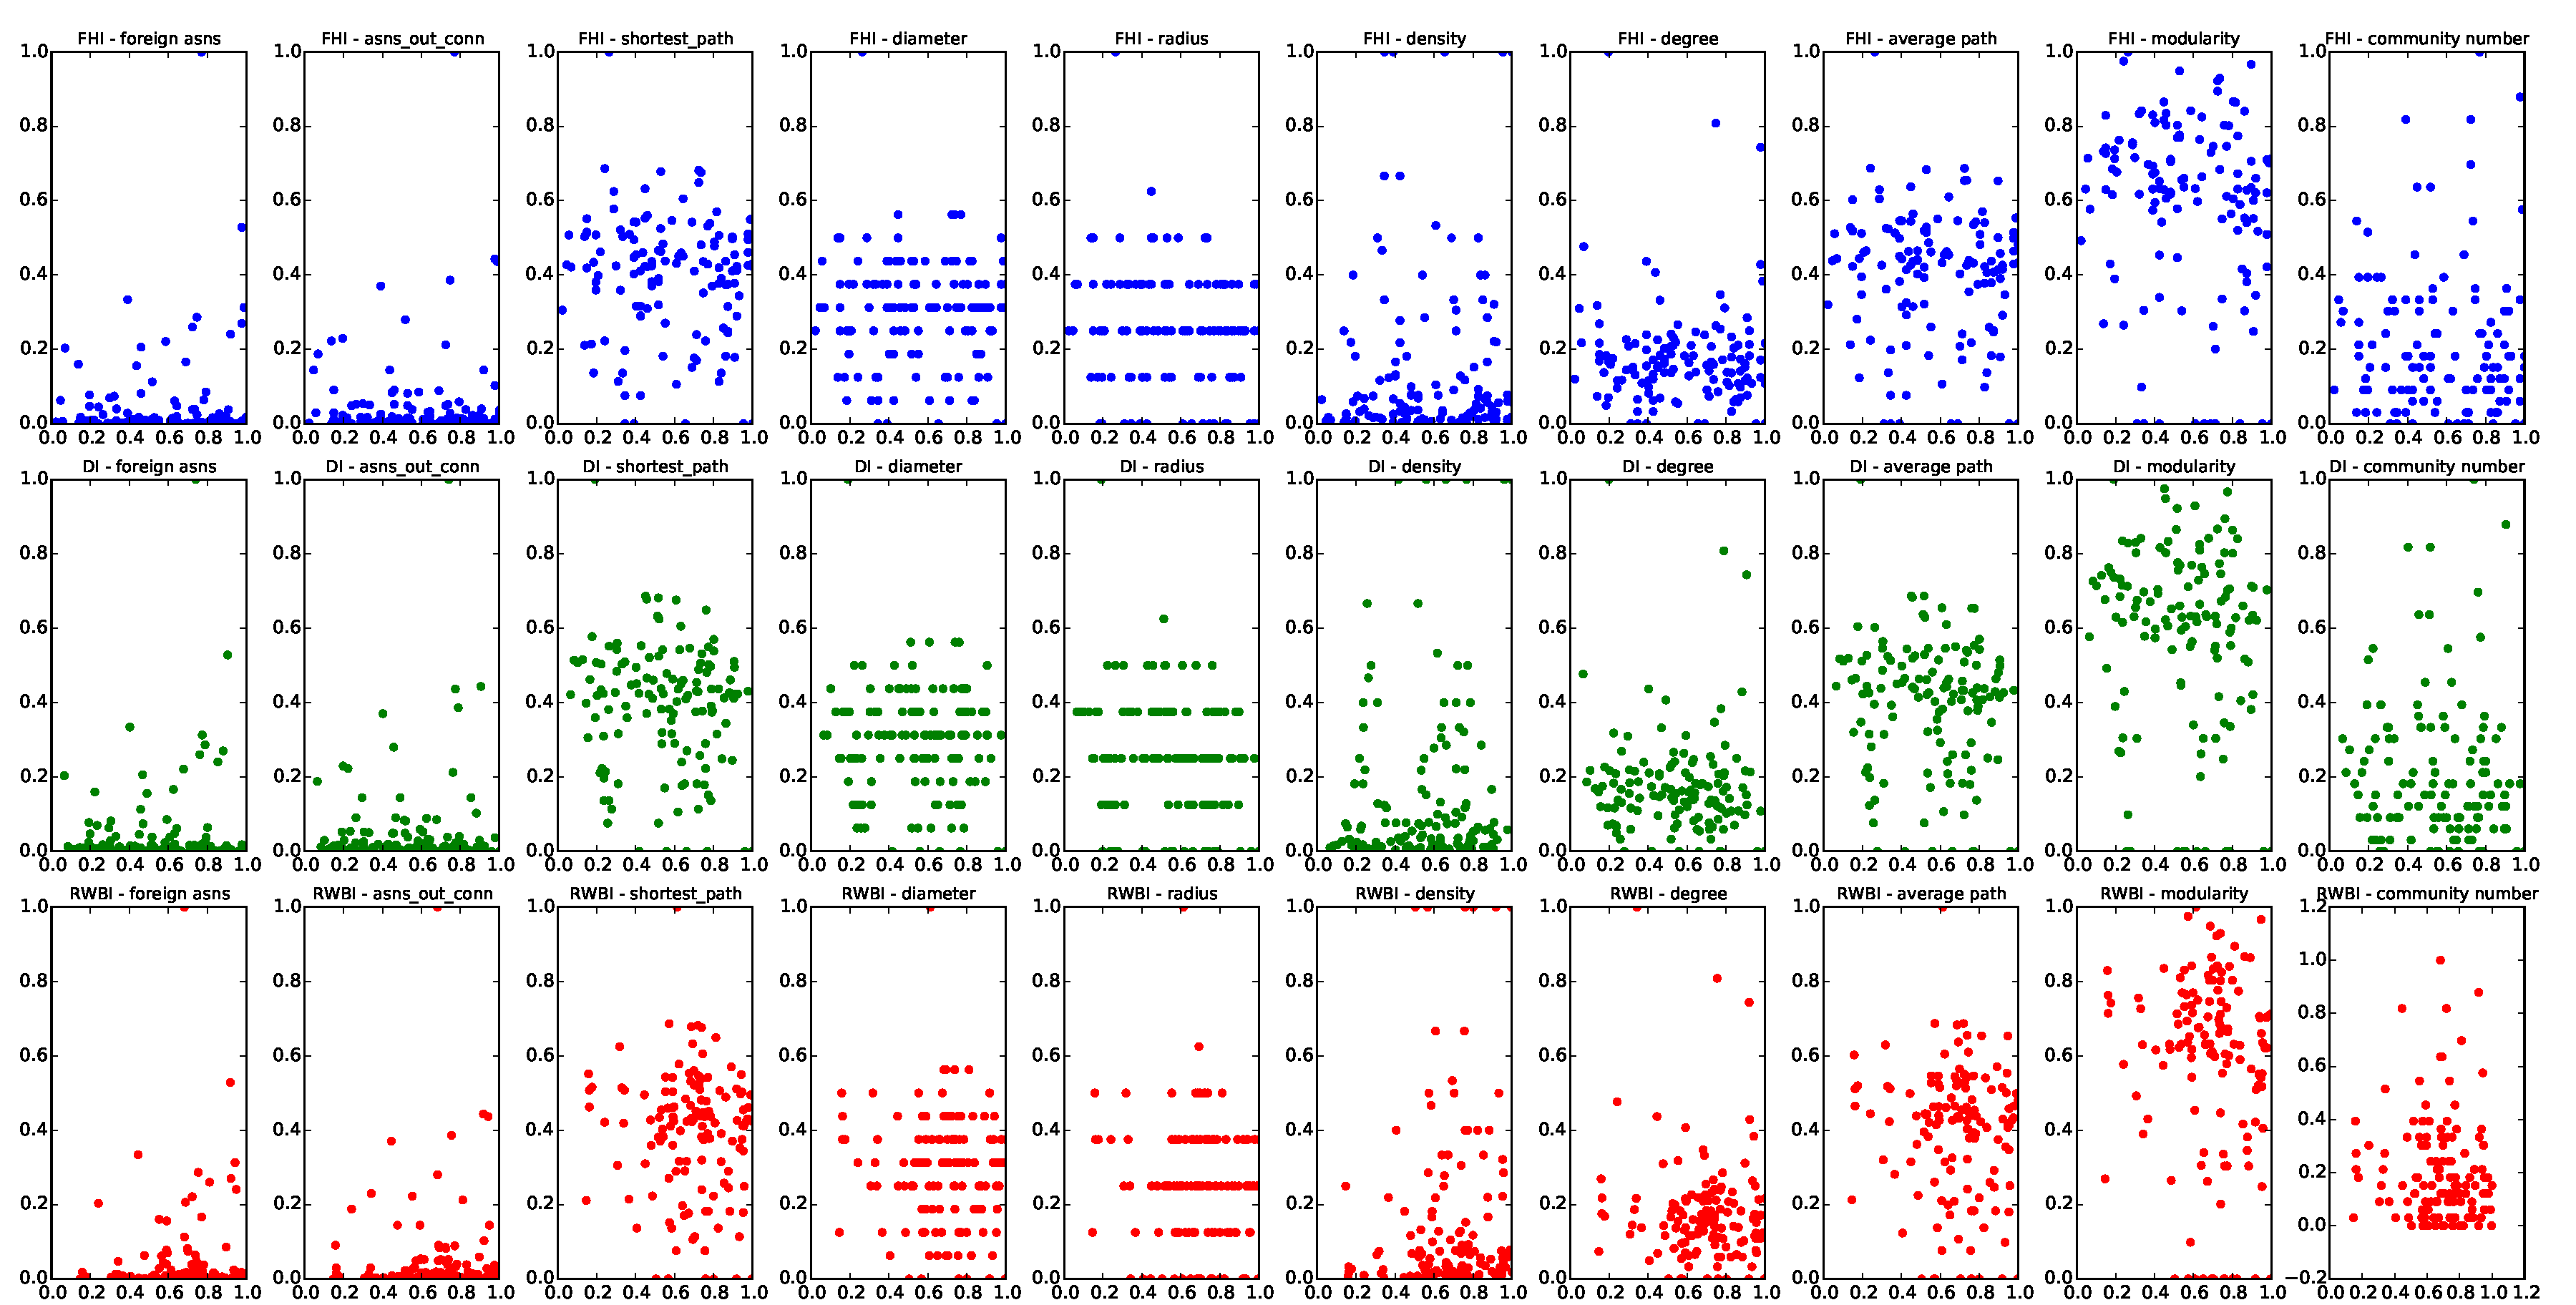
\includegraphics[width=0.97\columnwidth]{index_metric_scatter.pdf}
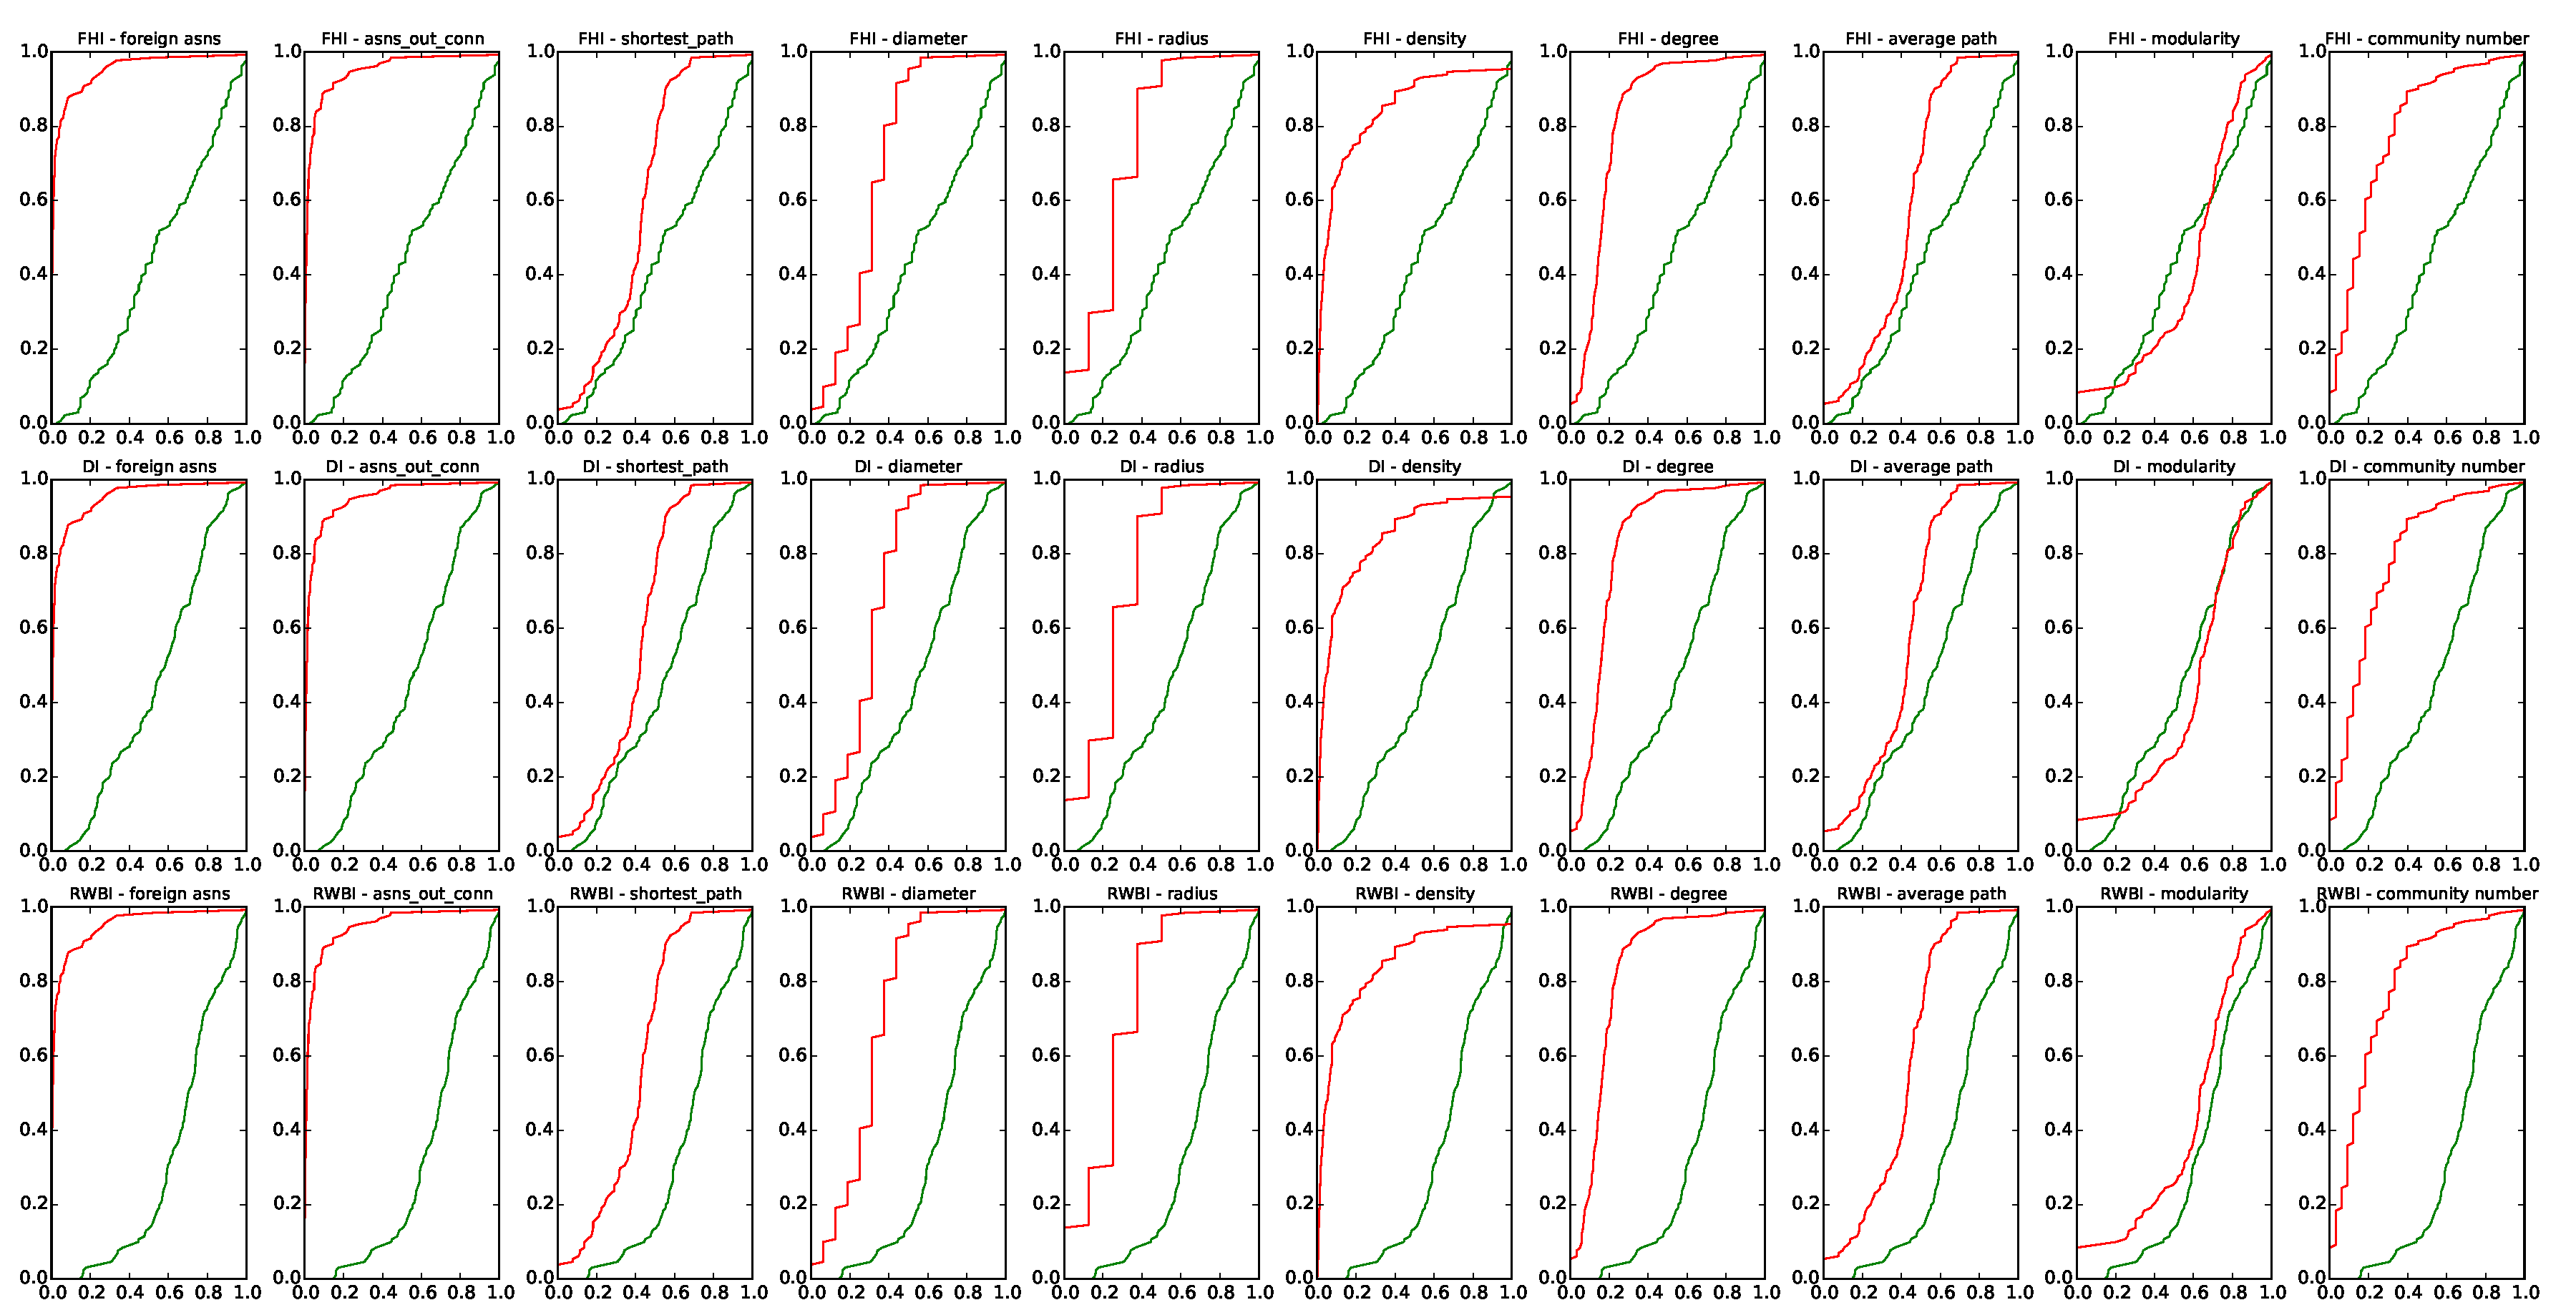
\includegraphics[width=0.97\columnwidth]{index_metric_cdf.pdf}
\caption{The scattering and CDF plot between the index and the metric}
\label{fig:im_scatter}
\end{figure}

\begin{figure}[h]
\centering 
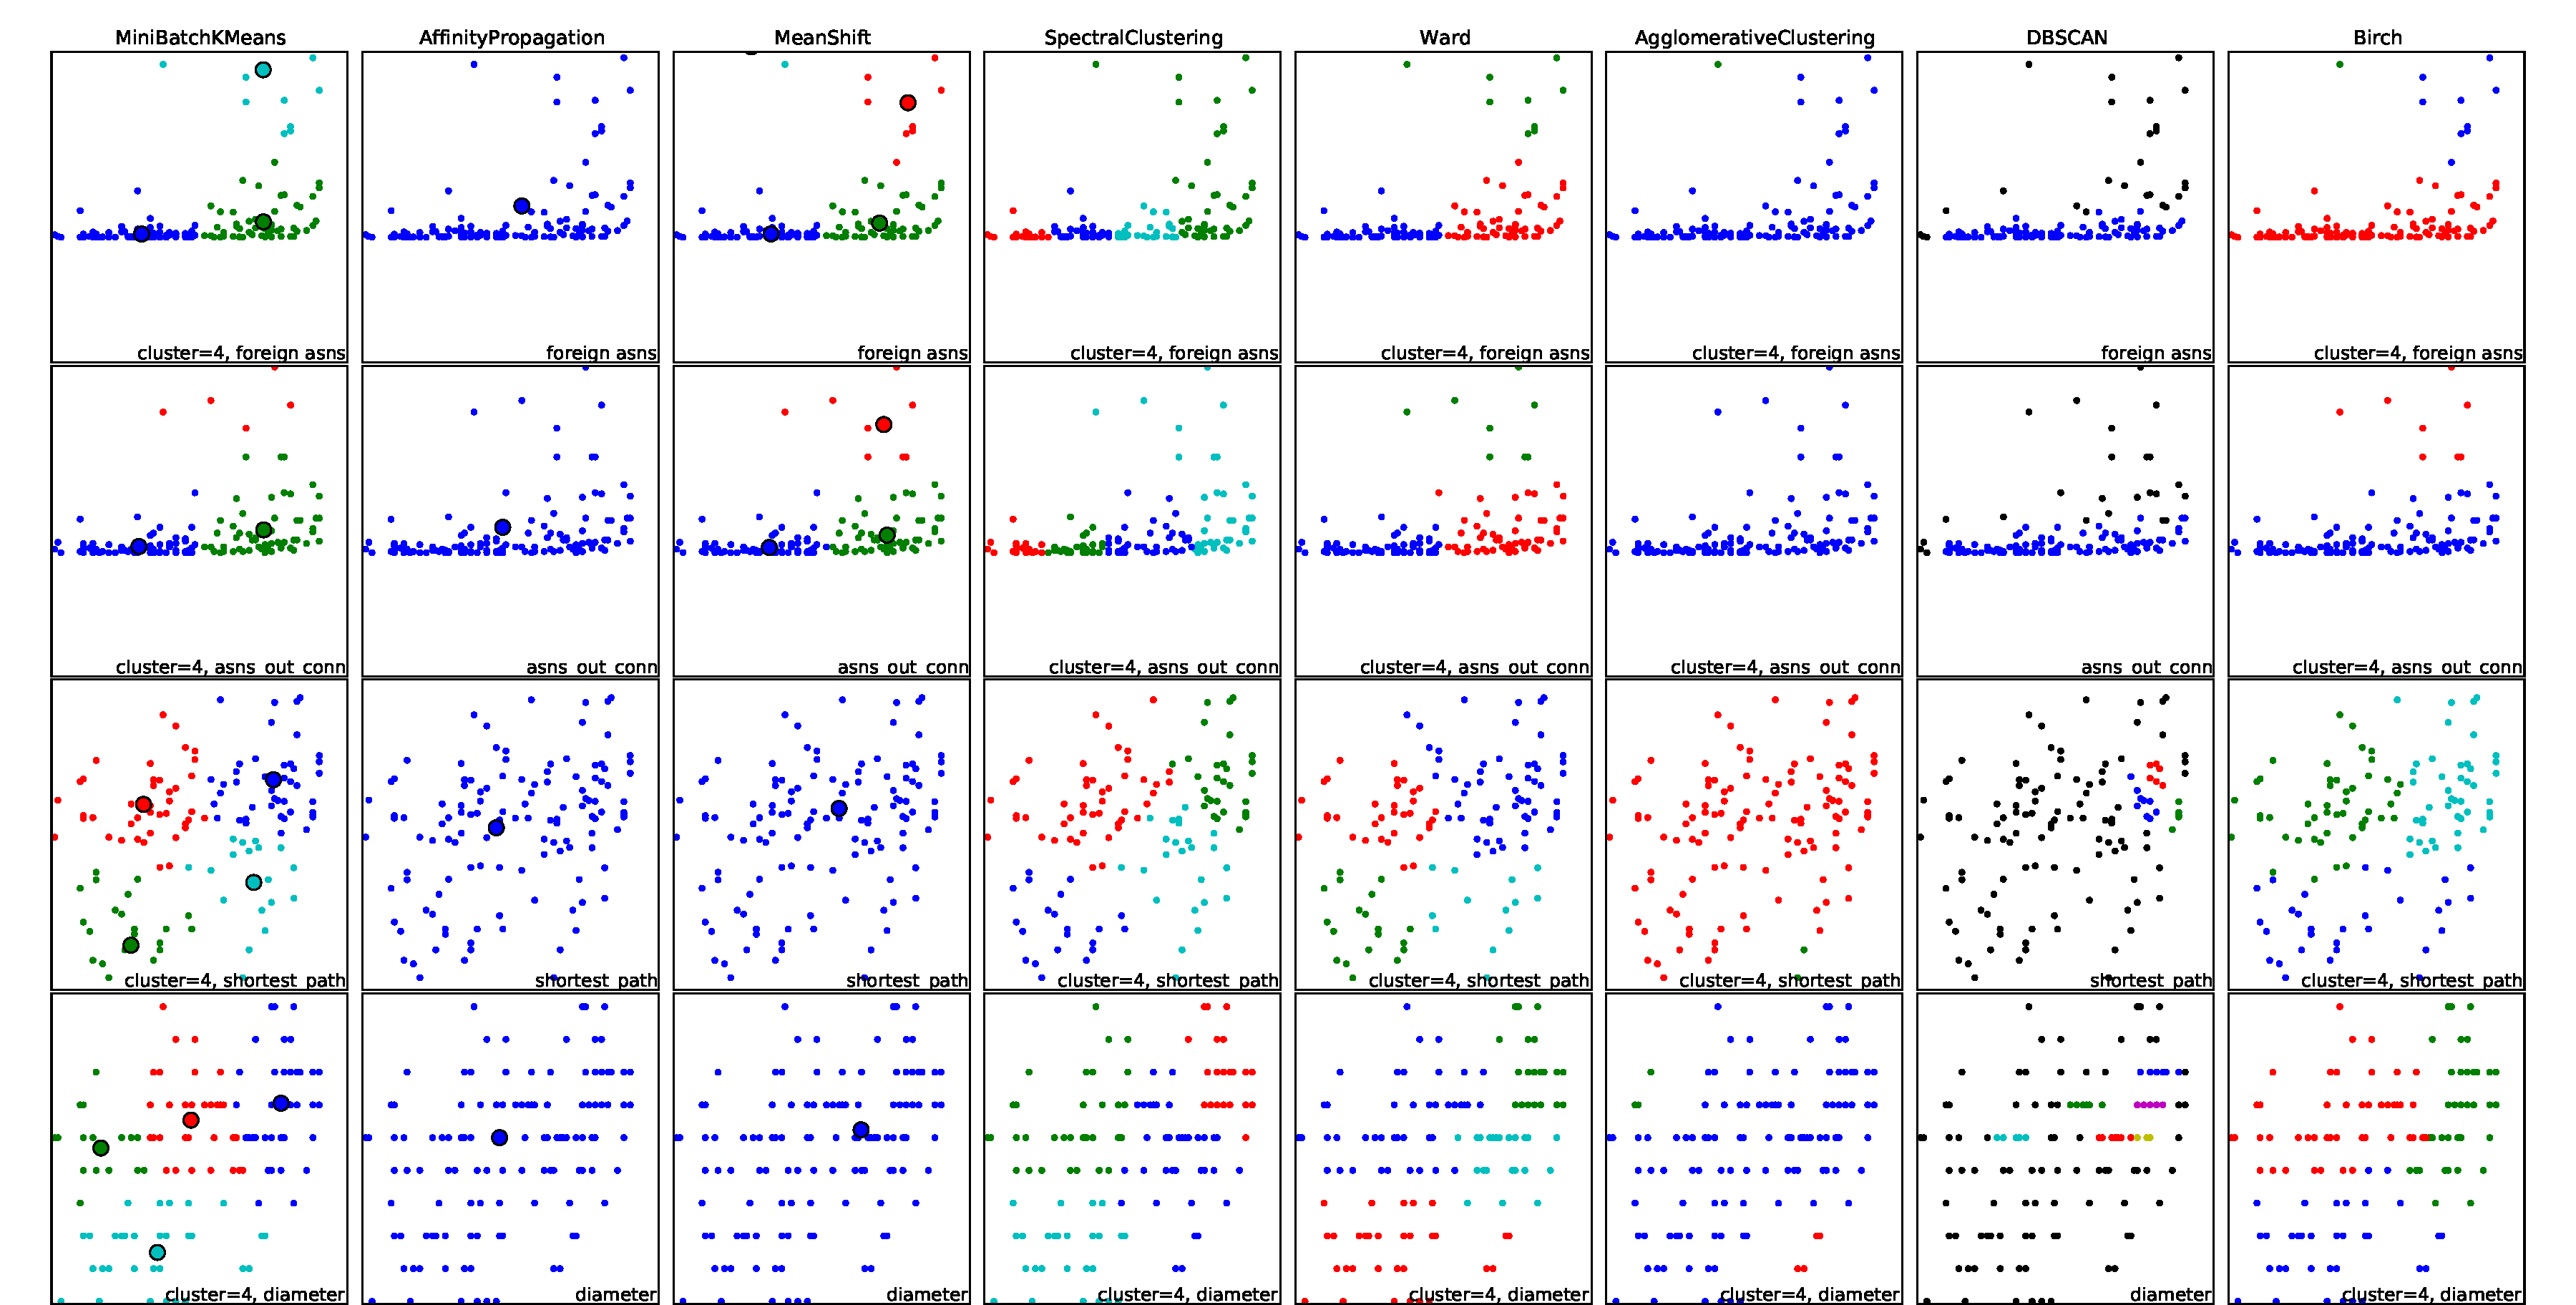
\includegraphics[width=0.97\columnwidth]{clustering_4_1.pdf}
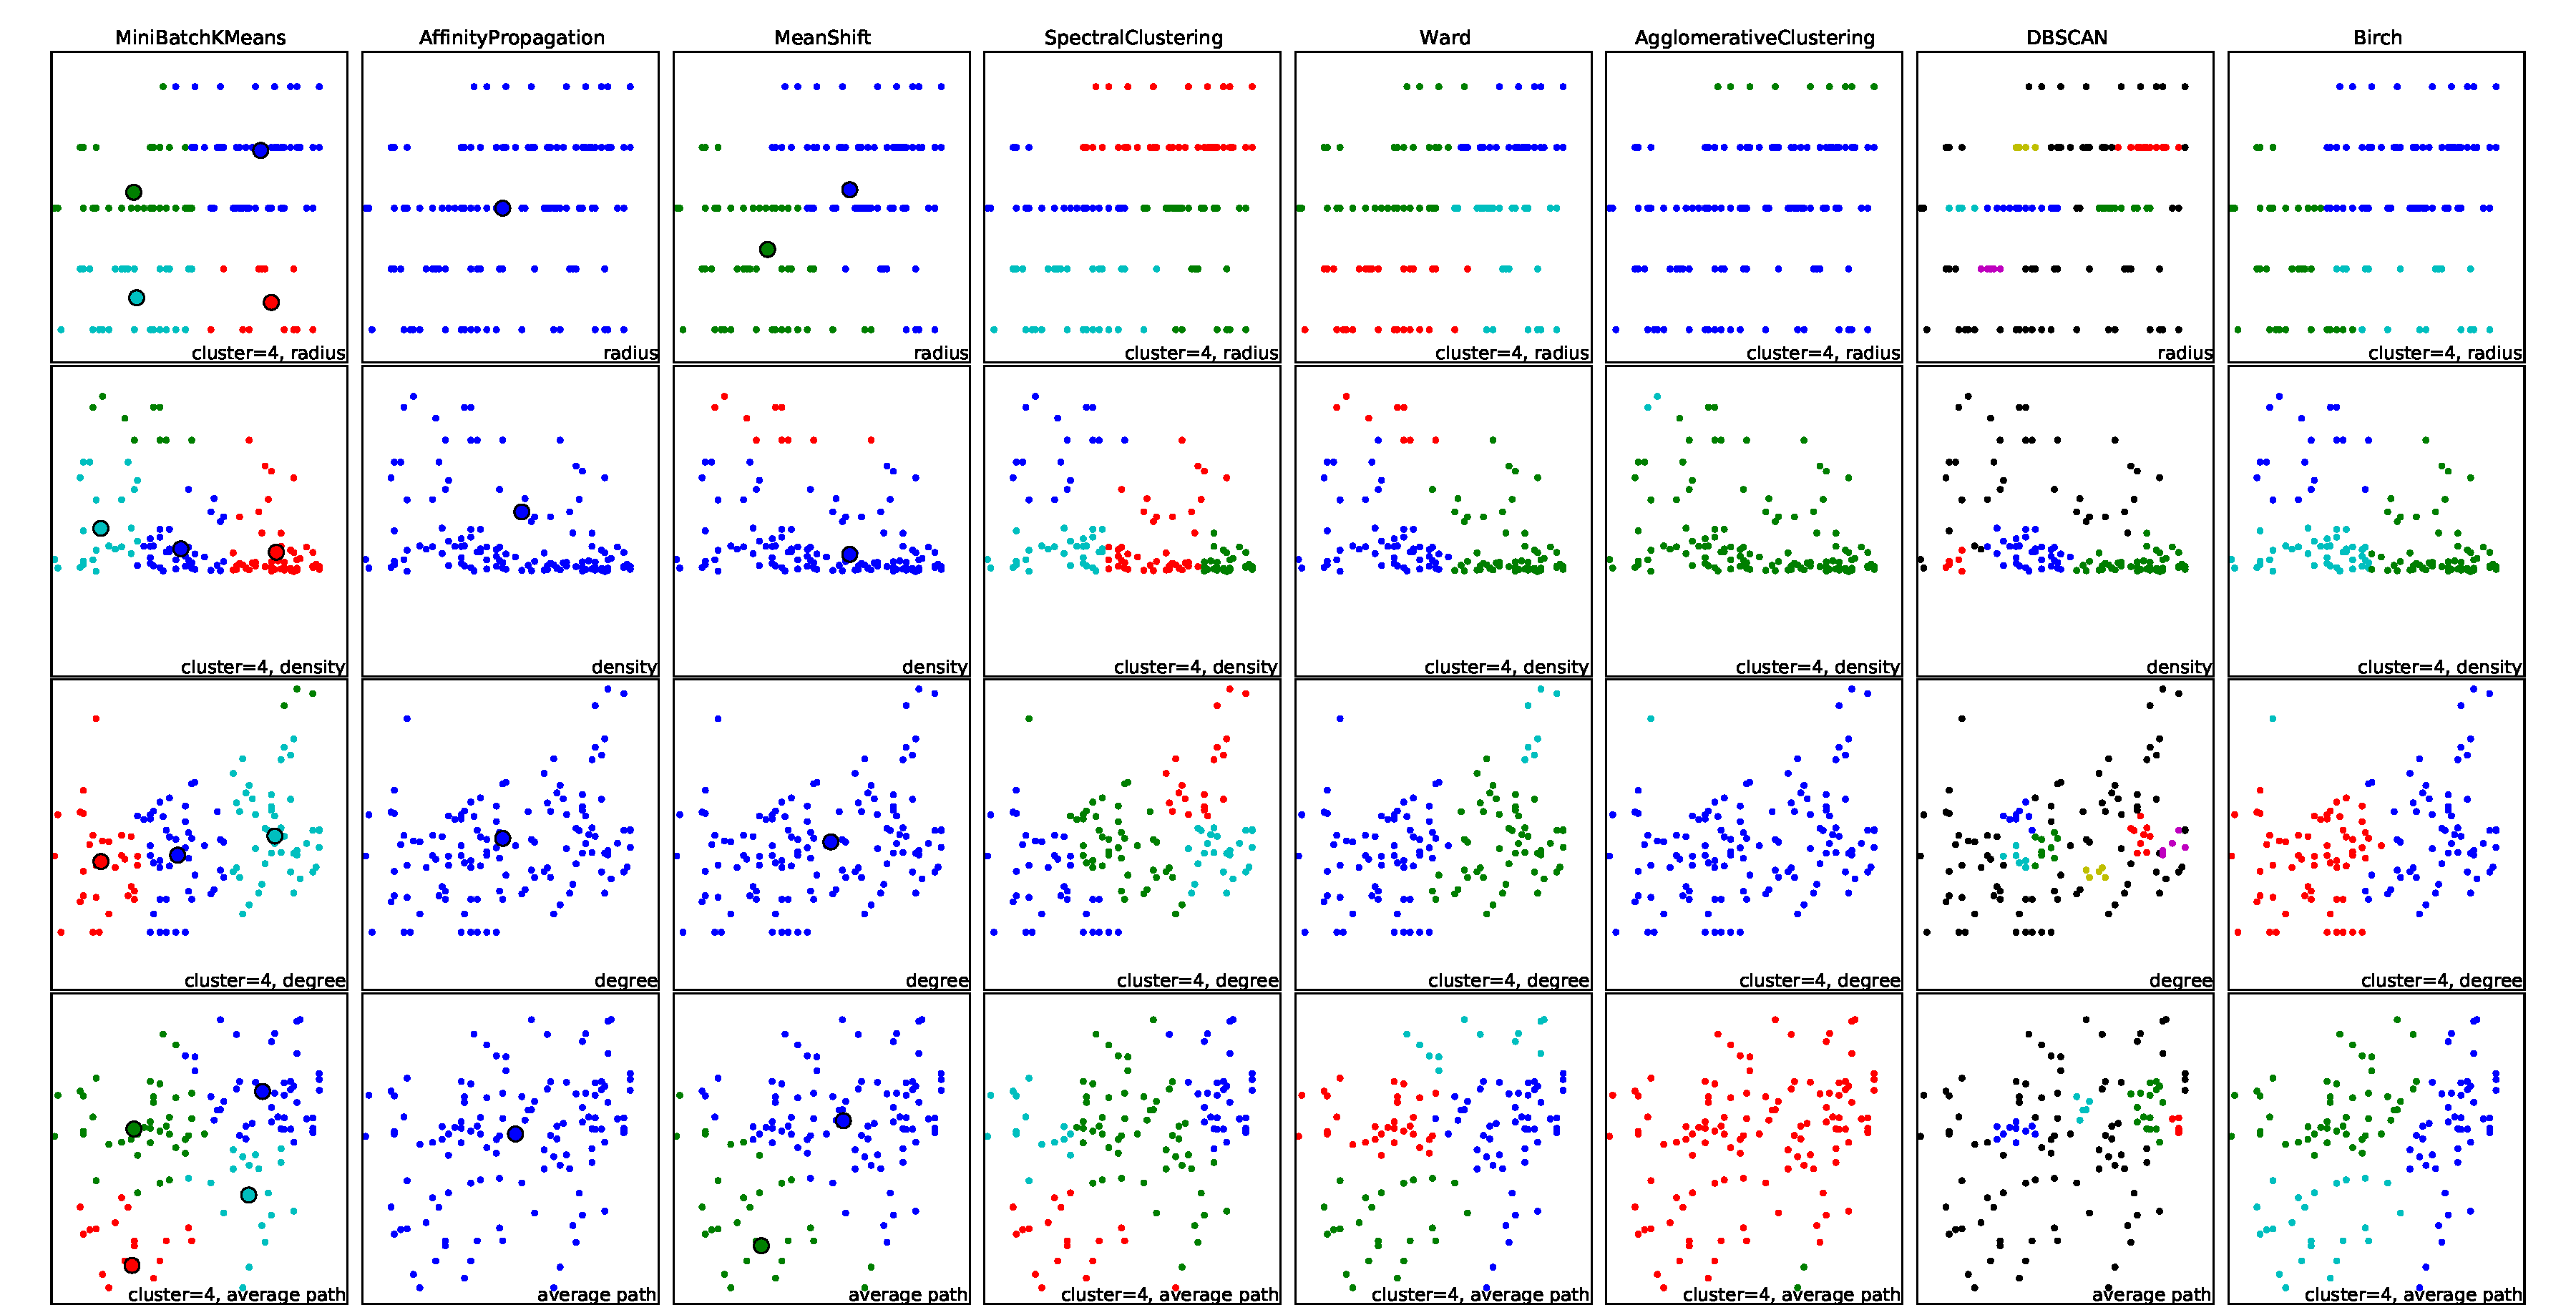
\includegraphics[width=0.97\columnwidth]{clustering_4_2.pdf}
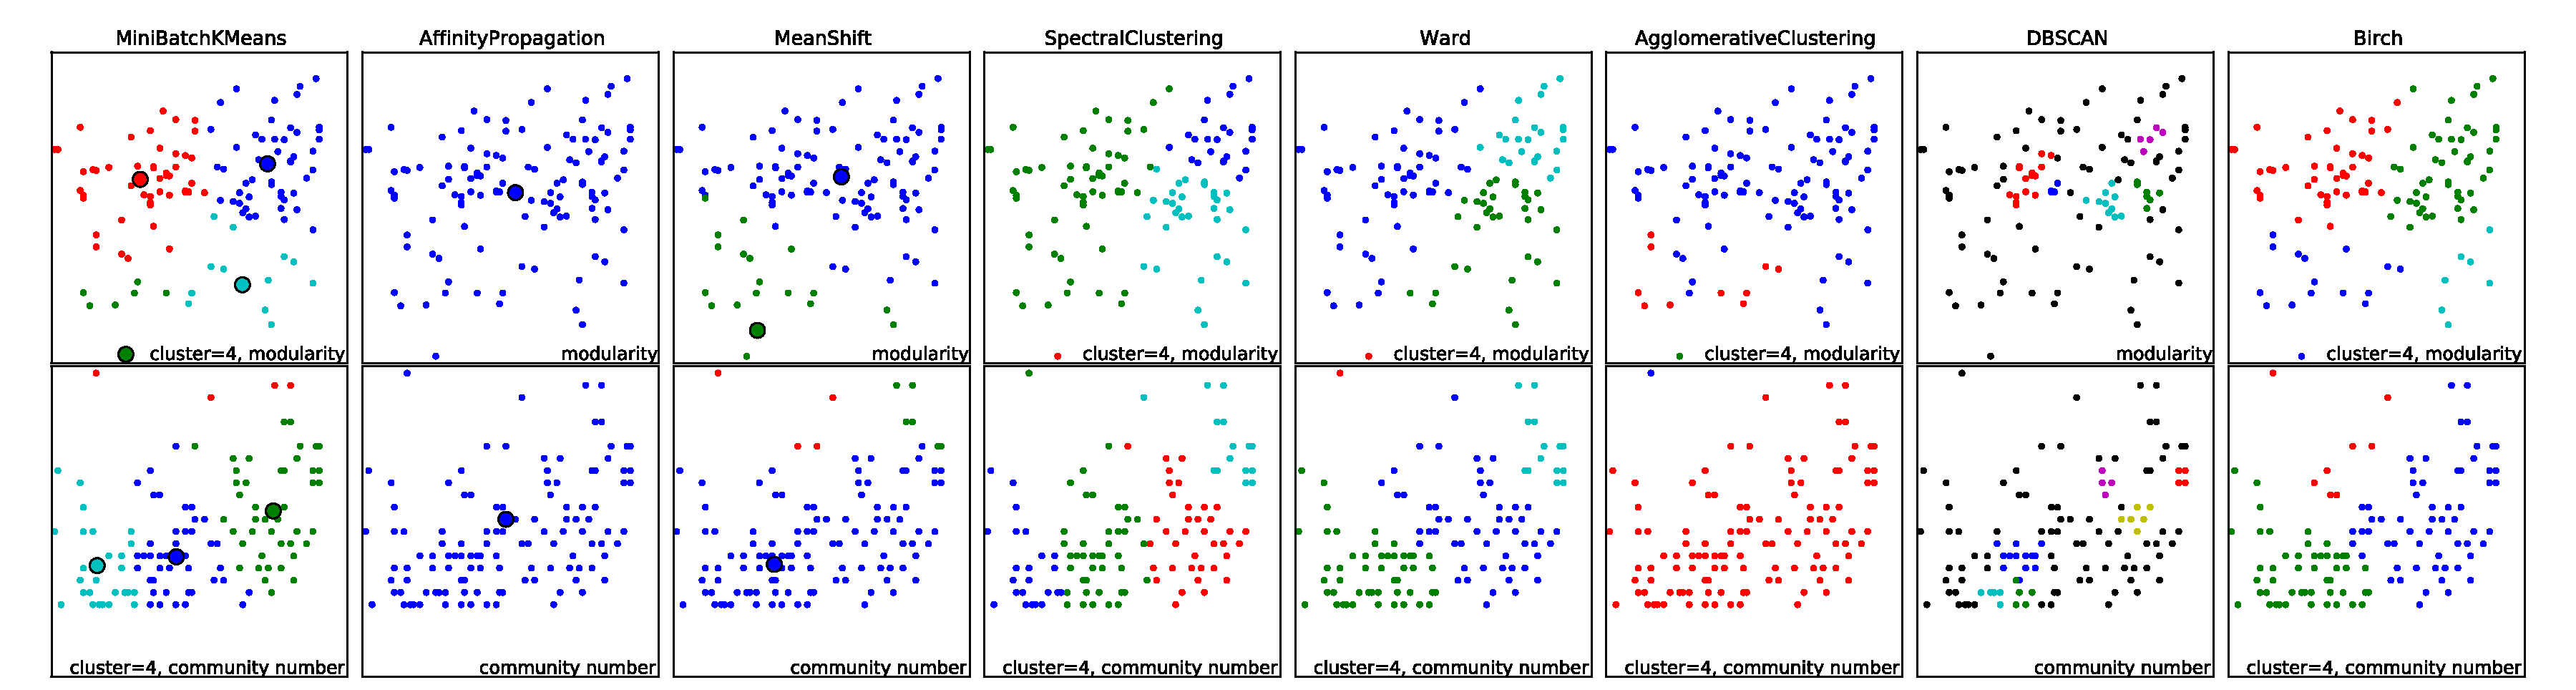
\includegraphics[width=0.97\columnwidth]{clustering_4_3.pdf}
\caption{Clustering example with four clusters}
\label{fig:clustering}
\end{figure}

\begin{table}
\centering
\caption{Number of ASes and the normalized indexes: Freedom House Index, Democracy Index and Reporters Without Borders Index)}
\label{tab:data}
\begin{longtable}{|l|l|l|l|l|l|l|}
\hline
No  & Country Code & Country Name                                         & ASNs  & FHI    & DI     & RWBI   \\ \hline
1   & AD           & Andorra                                              & 1     & 0.9655 & N/A    & 0.8403 \\ \hline
2   & AE           & United Arab Emirates                                 & 55    & 0.2874 & 0.1763 & 0.6223 \\ \hline
3   & AF           & Afghanistan                                          & 35    & 0.2644 & 0.1910 & 0.6131 \\ \hline
4   & AG           & Antigua and Barbuda                                  & 3     & 0.6782 & N/A    & 0.8254 \\ \hline
5   & AI           & Anguilla                                             & 2     & N/A    & N/A    & N/A    \\ \hline
6   & AL           & Albania                                              & 39    & 0.5287 & 0.5186 & 0.7252 \\ \hline
7   & AM           & Armenia                                              & 51    & 0.3678 & 0.3446 & 0.7296 \\ \hline
8   & AO           & Angola                                               & 33    & 0.3448 & 0.2565 & 0.6080 \\ \hline
9   & AQ           & Antarctica                                           & 0     & N/A    & N/A    & N/A    \\ \hline
10  & AR           & Argentina                                            & 376   & 0.5402 & 0.6508 & 0.7596 \\ \hline
11  & AS           & American Samoa                                       & 2     & N/A    & N/A    & N/A    \\ \hline
12  & AT           & Austria                                              & 423   & 0.8736 & 0.8429 & 0.9569 \\ \hline
13  & AU           & Australia                                            & 1169  & 0.8736 & 0.8960 & 0.8770 \\ \hline
14  & AW           & Aruba                                                & 2     & N/A    & N/A    & N/A    \\ \hline
15  & AX           & Åland Islands                                        & 1     & N/A    & N/A    & N/A    \\ \hline
16  & AZ           & Azerbaijan                                           & 36    & 0.1954 & 0.1977 & 0.3420 \\ \hline
17  & BA           & Bosnia and Herzegovina                               & 31    & 0.5632 & N/A    & 0.7415 \\ \hline
18  & BB           & Barbados                                             & 6     & 0.8966 & 0.4181 & N/A    \\ \hline
19  & BD           & Bangladesh                                           & 227   & 0.5172 & 0.5311 & 0.5419 \\ \hline
20  & BE           & Belgium                                              & 198   & 0.9885 & 0.7740 & 0.9423 \\ \hline
21  & BF           & Burkina Faso                                         & 6     & 0.6322 & 0.3401 & 0.7896 \\ \hline
22  & BG           & Bulgaria                                             & 526   & 0.7011 & 0.6384 & 0.6717 \\ \hline
23  & BH           & Bahrain                                              & 19    & 0.1494 & 0.2023 & 0.3384 \\ \hline
24  & BI           & Burundi                                              & 11    & 0.2874 & 0.2542 & 0.5422 \\ \hline
25  & BJ           & Benin                                                & 7     & 0.7241 & 0.5164 & 0.7192 \\ \hline
26  & BL           & Saint Barthélemy                                     & 0     & N/A    & N/A    & N/A    \\ \hline
27  & BM           & Bermuda                                              & 10    & N/A    & N/A    & N/A    \\ \hline
28  & BN           & Brunei Darussalam                                    & 6     & 0.2529 & N/A    & 0.6219 \\ \hline
29  & BO           & Bolivia, Plurinational State of                      & 15    & 0.5747 & 0.5322 & 0.6927 \\ \hline
30  & BQ           & Bonaire, Sint Eustatius and Saba                     & 0     & N/A    & N/A    & N/A    \\ \hline
31  & BR           & Brazil                                               & 3052  & 0.6092 & 0.7119 & 0.6844 \\ \hline
32  & BS           & Bahamas                                              & 4     & 0.8851 & N/A    & N/A    \\ \hline
33  & BT           & Bhutan                                               & 5     & 0.4483 & 0.4282 & 0.6751 \\ \hline
34  & BV           & Bouvet Island                                        & 0     & N/A    & N/A    & N/A    \\ \hline
35  & BW           & Botswana                                             & 14    & 0.6552 & 0.7672 & 0.8010 \\ \hline
36  & BY           & Belarus                                              & 87    & 0.0460 & 0.2949 & 0.4769 \\ \hline
37  & BZ           & Belize                                               & 9     & 0.8736 & N/A    & 0.8575 \\ \hline
38  & CA           & Canada                                               & 1084  & 0.8966 & 0.9040 & 0.9551 \\ \hline
39  & CC           & Cocos (Keeling) Islands                              & 0     & N/A    & N/A    & N/A    \\ \hline
40  & CD           & Congo, the Democratic Republic of the                & 14    & 0.1609 & 0.0757 & 0.5243 \\ \hline
41  & CF           & Central African Republic                             & 2     & 0.4023 & 0.0463 & 0.6597 \\ \hline
42  & CG           & Congo                                                & 11    & 0.4828 & 0.2045 & 0.6705 \\ \hline
43  & CH           & Switzerland                                          & 534   & 0.9770 & 0.9051 & 0.9182 \\ \hline
44  & CI           & Côte d'Ivoire                                        & 7     & 0.3103 & 0.2768 & 0.7035 \\ \hline
45  & CK           & Cook Islands                                         & 1     & N/A    & N/A    & N/A    \\ \hline
46  & CL           & Chile                                                & 145   & 0.7586 & 0.7593 & 0.7998 \\ \hline
47  & CM           & Cameroon                                             & 12    & 0.3333 & 0.2633 & 0.5848 \\ \hline
\end{longtable}
\end{table}

\begin{thebibliography}{9}
\bibitem{cymru} 
Team Cymru, IP to ASN Mapping,
\\\texttt{https://www.team-cymru.org/IP-ASN-mapping.html}
 
\bibitem{scikit} 
Scikit-learn, Clustering,
\\\texttt{http://scikit-learn.org/stable/modules/clustering.html}
 
\bibitem{censorship} 
Wikipedia: Censorship by country,
\\\texttt{https://en.wikipedia.org/wiki/Censorship\_by\_country}

\bibitem{caida}
CAIDA, AS Relationships Dataset,
\\\texttt{http://www.caida.org/data/as-relationships}

\bibitem{gephi}
Gephi, The Open Graph Viz Platform,
\\\texttt{https://gephi.org/}

\bibitem{networkx}
NetworkX, High-productivity software for complex networks,
\\\texttt{https://networkx.github.io/}

\bibitem{matplotlib}
Matplotlib, a python 2D plotting library with MATLAB-like interface,
\\\texttt{http://matplotlib.org}

\bibitem{similarity}
Danai Koutra, Ankur Parikh, Algorithms for Graph Similarity and Subgraph Matching,
\\\texttt{https://www.cs.cmu.edu/\~{}jingx/docs/DBreport.pdf​}

\bibitem{fhi}
Freedom House Index,
\\\texttt{https://freedomhouse.org}

\bibitem{di}
Wikipedia: Democracy Index,
\\\texttt{https://en.wikipedia.org/wiki/Democracy\_Index}

\bibitem{rwbi}
Reporters Without Borders Index,
\\\texttt{https://rsf.org/index2014/en-index2014.php}

\bibitem{topologies}
ASN topologies per each country at a glance,
\\\texttt{http://dandylife.net/test/topologies}

\bibitem{corrcoef}
Correlationship Coefficient for Indexes VS Metrics,
\\\texttt{http://bit.ly/1m7IMji}

\end{thebibliography}

\end{document}
